By studying the specification we conclude that we will be needing
eight different states; one for each {}``circle''. For input we
need a control for the direction (clockwise or counter-clockwise)
and a reset switch.

For output we would at minimum need to specify the orientation and
the number of the current circle to be displayed. These are defined
as top,d1,d0 (d for digit).\\
\\
Following the specification flow, leaves us with the following
finite state machine.


\subsection{Finite State Machine}

%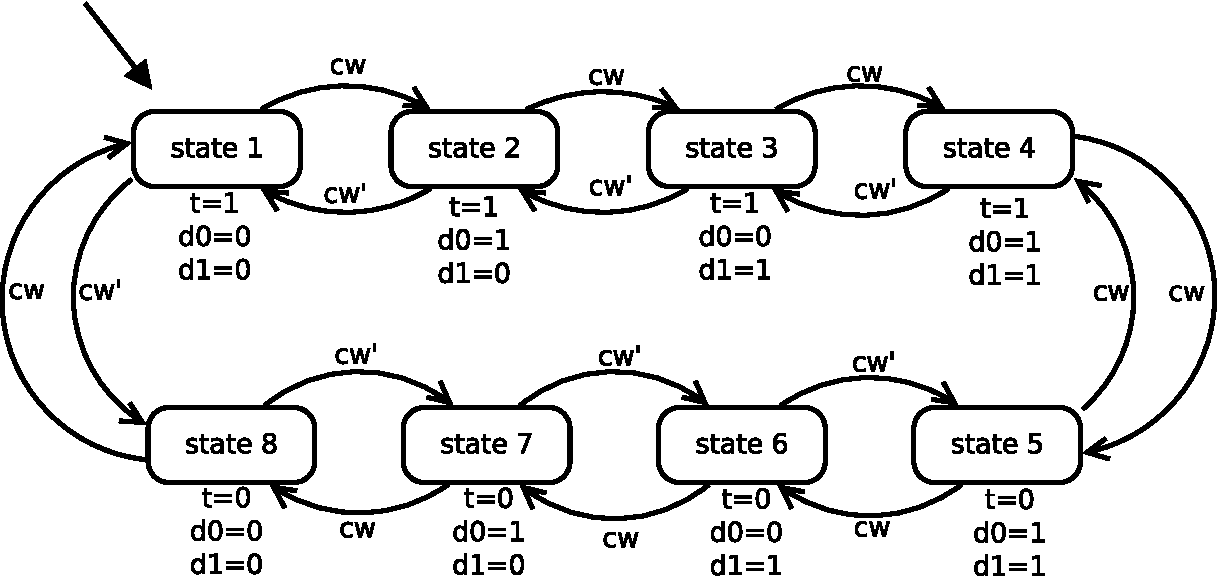
\includegraphics[width=0.7\textwidth]{fig/FSM_states.pdf}